%!TeX ts-program = xelatex
%!TeX encoding = utf-8 Unicode
\documentclass[ieeetran]{article}
\usepackage{amsmath, amssymb}
\usepackage{graphicx}

\title{Software Engineering for Business Applications Lecture Notes}
\author{Efe Kamasoglu}

\begin{document}

\maketitle

\pagebreak

\section{IT Support for Business Applications} % (fold)
\label{sec:iT_support_for_business_applications}

\subsection{Classification of Business Applications} % (fold)
\label{sub:classification_of_business_applications}

\begin{itemize}
  \item \textbf{Definition "Business Application":}
	  \begin{itemize}
	    \item \underline{in narrower sense:} totality of all programs, i.e.\ \textbf{application software}, and associated \textbf{data} for a concrete business use case
	    \item \underline{in broader sense:} additionally \textbf{hardware}, \textbf{system software} and necessary \textbf{communication} facilities required for the use of application software
	  \end{itemize}
\item \textbf{Two roles of Business Applications:}
	\begin{itemize}
	  \item \textbf{supporting}, \textbf{improving} or \textbf{automating} existing operational processes in bookeeping, accounting, etc.\ (size, speed, correctness...)
	\item \textbf{enabling} new products and services (e.g.\ online shopping and banking)
	\end{itemize}
\item \textbf{Classification of Business Applications by Business Purpose:}
	\begin{figure}[h!]
	  \centering
	  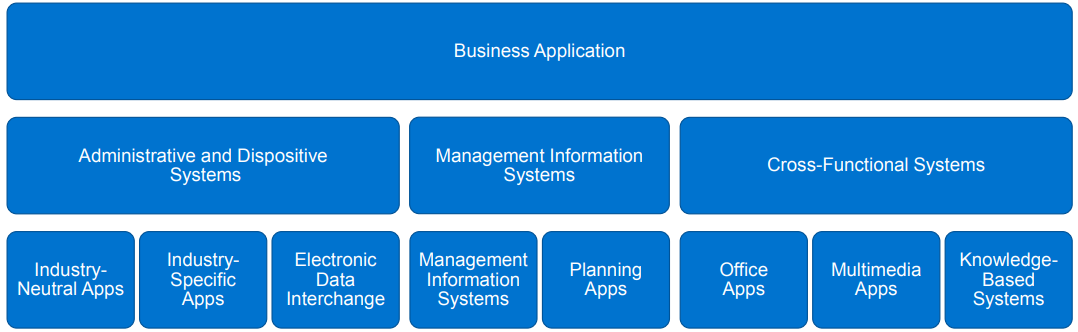
\includegraphics[width=0.5\linewidth]{classofba.png}
	  \label{fig:classofba_png}
	\end{figure}

\textit{\underline{Examples of}}

\begin{itemize}
  \item \textbf{administrative systems:} financial accounting, payroll accounting, administration of stocks
\item \textbf{disposition systems:}\ calculation and cost accounting, material procurement, field service control
\item \textbf{management information systems (MIS):} use of internal company data, use of external data, combination of multiple data sources in a flexible form
\item \textbf{planning systems:}\ planning of individual functional areas, integrated planning of several functional areas, corporate planning

\end{itemize}
\item \textbf{Cross-Cutting Applications:}
	\begin{itemize}
	  \item independent of company hierarchy and fuctional domains
	\item used either directly via user interface or programmatically via administration and disposition systems
	\item \textit{Examples:} office suites, groupware, workflow management systems
	\end{itemize}

\item \textbf{Enterprise Resource Planning (ERP):} \textbf{ERP system} is an integrated business application (suite, collection of programs), which supports all essential functions of administration, disposition and management with a \underline{common interface and a shared and integrated data management}.
	\begin{itemize}
	  \item consists of platform and function-oriented application components that exchange info and events
          \item is realized as (customizable) standard software
	\item \textit{Examples:} external accounting, controlling, procurement
	\item Today's ERP systems support an \textbf{extended value chain}\footnote{\textbf{Value chain} is a business model that describes the full range of activities needed to create a product or service.}.
	\end{itemize}
\end{itemize}

\subsection{Standard and Custom Software} % (fold)
\label{sub:standard_and_custom_software}

\begin{itemize}
  \item \textbf{Standard Software vs. Custom Software:}
	  \begin{itemize}
	    \item \textbf{Standard software} \textit{(e.g.\ SAP)}
		    \begin{itemize}
		      \item developed for specific \textbf{market}
		\item distributed by a software house
			\item can be used by \textbf{several companies}
			\item implements "standard business processes" at its core
			\item maintained by \textbf{manufacturer}, adapted to changes
			\item must or can be \textbf{customized} to company (e.g.\ authorizations and roles, currencies) 
		    \end{itemize}
	\item \textbf{Custom software}
		\begin{itemize}
		  \item specifically developed for \textbf{one company}
	\item tailored to specific business processes/requirements
		\item result of a project for a known client
			\item \textbf{individually} maintained and adapted to changes
		\end{itemize}
	  \end{itemize}
\pagebreak
\item \textbf{Adaptation Techniques for Standard Business Software:}
	\begin{itemize}
		\item Adaptation of operational standard software can be divided into \textbf{Configuration}, \textbf{Extension} and \textbf{Coupling} (= \textbf{Customizing}).
               \begin{figure}[h!]
                 \centering
                 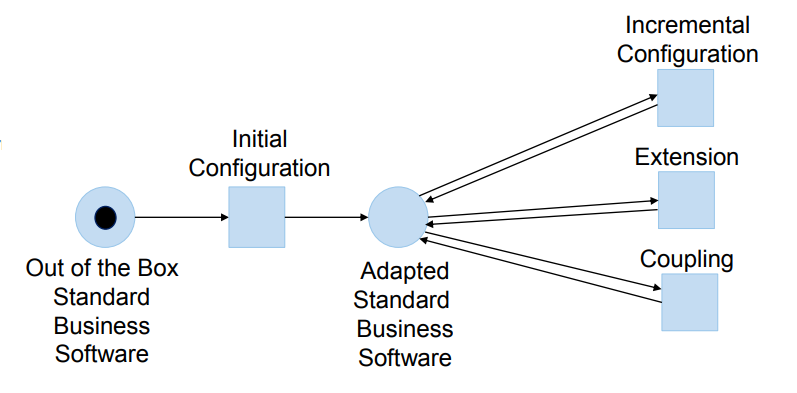
\includegraphics[width=0.5\linewidth]{adaptationsbs.png}
                 \label{fig:adaptationsbs_png}
               \end{figure} 

	       \item \textbf{Configuration} describes functionalities and techniques
		       \begin{itemize}
		         \item that are obligatory on first deployment
				 \item that allow to define predefined settings
			\item that lead to an individual variation of standard software
		       \end{itemize}

	\item \textbf{Extension} describes functionalities and techniques
		\begin{itemize}
		  \item that are optional for productive use
			  \item that allow to map requirements not foreseen by manufacturer
				  \item implemented by manufacturer to expand the range of services
		\end{itemize}

		\item \textbf{Coupling} refers to functionalities and techniques
			\begin{itemize}
			  \item to connect external systems of other manufacturers
				  \item to connect external systems of the same type
				\item that are predefined in the form of data file formats, APIs, or communication protocols
			\end{itemize}


		\item \textit{Example:} mapping the structure of a company to SAP applications via organizational units (can be assigned to single or multiple apps)
	\end{itemize}

	\item \textbf{Configuration: Challenges}
		\begin{itemize}
		  \item A \textbf{standard software} must
			  \begin{itemize}
			    \item provide all relevant configuration options
			\item support a wide range of different corporate structures and processes
			\item check dependencies between these many variants
			\item provide appropriate documentation about the effects of individual configurations

			  \end{itemize}
		  \item \textbf{Consequences:} 
				  \begin{itemize}
				    \item need for experts who are familiar with configuration options of each release and componant
					   \item scarcity of such experts
						   \item expensive training
							   \item expensive consultancy services
				  \end{itemize}
		\end{itemize}

\item \textbf{Examples for Extensions:}
	\begin{itemize}
	  \item automation of \textbf{multi-step business workflows}
	\item integration of company-specific calculations/rules/checks
	\item connecting customers
	\end{itemize}
\item \textbf{Coupling Options:}
	\begin{itemize}
	  \item different coupling options depending on the scenario
	\item programming language used for coupling
	\item available mechanisms to couple
	\end{itemize}

\item \textbf{Multi Tenancy:} Software multitenancy is a software architecture in which a single instance of software runs on a server and serves multiple tenants (e.g.\ companies).
	\begin{itemize}
	  \item several companies can be represented in one system
	\item distinction between tenant-dependent and -independent data
	\item supporting tenant-dependent authorization (e.g.\ A may only perform transactions in client 002)
         \item individual adaptations of tenants (e.g.\ currency, couplings)
	\end{itemize}

\item \textbf{Multilingualism:}

	\begin{itemize}
	\item \textbf{Multilingualism of a business information system} makes it possible to
		\begin{itemize}
		  \item store and display texts in different languages in the system
		\item assigning graphics and symbols specific to different languages 
		\end{itemize}
	
\item Multilingualism requires
	\begin{itemize}

\item that one system can process all relevant character sets at once
	\item storage and recognition of words, numbers etc.
	\item that a system can assign users to languages or user can choose their own
	\item that texts (graphics, symbols) can be assigned to a language
	\end{itemize}
	\end{itemize}
\item \textbf{Localization (l10n):} Adaptation of a software product to meet the language, culture, and other requirements of each locale (e.g.\ adaptation of graphics, currencies, date and time)
\item \textbf{Internationalization (i18n):}\ Process of preparing a software-based product for localization (to support global markets)
\end{itemize}

\subsection{Characteristics of Business Applications} % (fold)
\label{sub:characteristics_of_business_applications}
\begin{itemize}
  \item \textbf{Multiple Stakeholders and changing requirements:}
	  \begin{itemize}
	    \item \textbf{Requirements Elicitation and Requirements Management}
		    \begin{itemize}
		      \item many stakeholders, different views and concerns
		\item Waterfall: upfront requirements document and/or technical specification => Req. Documentation
		\item Issue: changing requirements once IT support is implemented
		\item Agile: incremental and iterative => Agile Req. Engineering
			\item typically, very large number of requirements
			\item need for formalization and early consistency checking => Conceptual Modeling
				\item need for cost and time prediction => Software Estimation

		    \end{itemize}

	\item \textbf{Programming Challenges}
		\begin{itemize}
		  \item design, implement and test changes in an existing complex system => Change Mgmt.
	\item deliver incremental changes without invalidating existing data => Release Mgmt.
		\item parallel development at manufacturer and at customer site => Version Mgmt.

		\item automated and quality-controlled assembly of application software => Build Mgmt.
		\end{itemize}
	  \end{itemize}

\item \textbf{Persistent Data and Concurrent Data Modification:}
	\begin{itemize}
	  \item \textbf{Data consistency} is a must:
		  \begin{itemize}
		    \item many users perform \textbf{transactions} simultaneously on central databases
		\item data must not be lost even in case of system failures
		  \end{itemize}
		  \item \textbf{Programming challenges:}
			  \begin{itemize}
			    \item database is managed by an independent application, on a different server / hardware
			\item object orientation is not supported by common data bases
				\item database concepts must be transferred to the application logic (transactions, rights, primary keys)
			  \end{itemize}
	\end{itemize}

\item \textbf{Distributed Actors and Data Repositories:}
	\begin{itemize}
	  \item \textbf{Many users access central data concurrently:}
		  \begin{itemize}
		    \item users need data in different locations at different times
			    \item Client-Server architecture => Layered Architectures
		\item web clients => REST protocol
		  \end{itemize}

	\item \textbf{Programming challenges:}
		\begin{itemize}
		  \item software components must be able to found in network => Naming services
		  \item communication always via a network => Serialization\footnote{\textbf{Serialization} is the process of translating a data structure into a format that can be stored or transmitted and reconstructed later.} \& failed execution
			  \item authentication and authorization => Security
		\item concurrent accesses => Transactions
		\end{itemize}
	\end{itemize}

\item \textbf{Integeration of Data and Application from (Semi-)Autonomous Sources:}
	\begin{itemize}
	  \item \textbf{Separation of applications and data repositories:}
		  \begin{itemize}
		    \item multiple apps work on independent or shared data resources
			    \item multiple apps communicate with each other => RPC, Message Passing
			\item business processes involve multiple apps => Workflow Mgmt. Systems
			\item application landscapes with lots of interacting applications => Enterprise Architecture Mgmt.
		  \end{itemize}

		  \item \textbf{Programming challenges:}
			  \begin{itemize}
				  \item integration of multiple languages and databases
				\item loose coupling through interfaces to avoid code change propagationi
				\item error recovery to avoid runtime failure propagation
			  \end{itemize}
	\end{itemize}

\item \textbf{Scalability:}
	\begin{itemize}
	  \item \textbf{Growing number of users and data volume}
		  \begin{itemize}
		    \item business apps are used by thousands of employees world-wide around the clock
		\item customers and business partners interact directly with business apps and expect real-time sub-second response times
		\item volatile load (e.g.\ online shop in christmas season vs.\ summer season)
		  \end{itemize}
		  \item \textbf{Programming challenges:}
			  \begin{itemize}
				  \item delayed execution of resource-intesive operations => Batch processing\footnote{\textbf{Batch processing} is when a computer processes a number of tasks that it has collected in a group. It is designed to be a completely automated process, without human intervention.}
				    \item dynamically increasing/decreasing number of users => Instance pools
					    \item single server cannot handle the load => Load balancing, Caching
		
			  \end{itemize}
	\end{itemize}
\end{itemize}

\section{Requirements Engineering} % (fold)
\label{sec:requirements_engineering}

\begin{itemize}

\item \textbf{Software requirements} express the needs and constraints placed on a software product.

  \item \textbf{Requirements engineering} is concerned with \textbf{elicitation}, \textbf{analysis}, \textbf{specification} and \textbf{validation} of software requirements as well as the management of requirements.

\item \textbf{Requirements Management} deals with the administration and maintenance of requirements documents, in particular:
	\begin{itemize}
	  \item change requirements (change management)
          \item trace and link requirements (requirements tracing)
	  \item verify requirements
	\end{itemize}


\end{itemize}

\subsection{Traditional Requirements Engineering} % (fold)
\label{sub:traditional_requirements_engineering}

\begin{itemize}
	\item \textbf{Objectives of Requirements Management:}
		\begin{itemize}
		  \item \textbf{Efficient} preparation of \textbf{high quality} requirements and system specifications,
			   \begin{itemize}
			     \item coordinated with all stakeholders (different objectives and interests)
			\item coordinated with all specifications and constraints
			\item evaluated according to profitability and feasibility 
			   \end{itemize}

		\item \textbf{Specification documents} are basis for:
			\begin{itemize}
			  \item contract negotiation and contractual agreements
		\item coordination between the stakeholders (customers, developers)
		\item design, realization, integration
			 \item software acceptance (test specification)
			\item future developments, projects
			\end{itemize}
		\end{itemize}
\item \textbf{Requirement Classification:} Distinction between \underline{functional and non-} \underline{functional requirements and constraints}:
	\begin{itemize}
		\item \textbf{Functional requirements} \ describe \underline{interactions} between the system and its environment independent of their realization.
		\item \textbf{Non-functional requirements} describe \underline{general properties} of the system.
\item \textbf{Restrictions (Constraints)} determine the \underline{solution space} for the realization.	
	\end{itemize}

\item \textbf{Stakeholder Management:} It includes
	\begin{itemize}
	  \item processes required to identify people that could impact or be impacted by the project
\item to analyze stakeholder expectations and their impact on the project
	\item to develop appropriate management strategies for effectively engaging stakeholders in project decisions and execution
	\end{itemize}

\item \textbf{Requirement Specification:}
	\begin{itemize}
	  \item technical result document of requirement identification phase
	\item \textbf{contains} \underline{stakeholder identification, functional and non-functional}\\ \underline{requirements, constraints, evaluation plan and metrics}
	\item list of all deliverables and services to be fulfilled by contractor within contract as defined by customer
	\item \textbf{what} is to expect from the solution (product)
	\item formulation of requirements should be as general as possible and as restrictive as necessary
	\item enables the contractor to develop optimal solutions
	\end{itemize}

\item \textbf{Requirements Validation:} \textbf{Validation}, \textbf{Consistency check} (no conflicts), \textbf{Completeness check}, \textbf{Reality check}, \textbf{Verifiability}

\item \textbf{Functional Specification:}
	\begin{itemize}
	\item defines the purpose of the system
	  \item solution proposal created by contractor based on the requirement specification provided by client
		  \item \textbf{contains} \underline{target determination, product usage, environment (e.g.}\\ \underline{hardware), functions, UI, global test cases} 
	\item system description or solution specification, which describes \textbf{how} the solutions is to be realized (concrete solution approaches)
	\item the \textbf{what} from \textbf{requirement specification} is detailed
	\end{itemize}
\end{itemize}

\subsection{Agile Requirements Engineering} % (fold)
\label{sub:agile_requirements_engineering}

\begin{itemize}
  \item \textbf{Requirements Engineering and Agile Software Development:}
\begin{itemize}
  \item \textbf{Agile software development} focuses more on \textbf{continuous collabration} (workshops, interviews etc.) with stakeholders instead of relying on \textbf{specification documents} (\textit{example: SCRUM})
	  \item \textbf{Traditional requirements engineering}
		  \begin{itemize}
		    \item focuses on customer collabration mainly at an \underline{early phase of the} \underline{project} (longer change cycles)
			   \item emphasizes a heavy-weight process with extensive, \textbf{static specification documents}
				   
		  \end{itemize}


\item \textbf{Agile requirements engineering}
	\begin{itemize}
		\item fosters communication with the customer during the \underline{whole development}\\ \underline{process} to \textbf{continuously update requirements}
		\item focuses less on extensive documentation, but specification documents \textbf{might be necessary} because of legal or contracting reasons etc.
		\item includes activities and artifacts that are similar to classical requirements engineering activities
	\end{itemize}
\end{itemize}

\item \textbf{Typical Requirement Artifacts in Agile Software Development:}
	\begin{itemize}
	  \item \textbf{user story}, \textbf{story card}, \textbf{use case}, \textbf{scenario}, \textbf{UML diagram}, \textbf{prototype}
	\end{itemize}

\item \textbf{User Stories:}
	\begin{itemize}
	  \item explanation of a software feature written from the perspective of the end user
		  \item most frequently used artifact in \textbf{agile software development}
		  \item mnemonic for writing good user stories: INVEST\footnote{independent, negotiable, valuable, estimable, small, testable}
	\end{itemize}

\item \textbf{Typical Requirements Engineering Challenges:}
	\begin{itemize}
	  \item different interest groups can raise \textbf{conflicting requirements}
	\item the people who \textbf{pay} for the system are rarely the ones who \textbf{use} it
	\item the organization and the technical environment may \textbf{change} after the system rollout
	\item requirements that change during implementation (Change Requests) can lead to additional costs -> project duration/milestones can be affected significantly
	\end{itemize}
\end{itemize}


\section{Conceptual Modeling with UML} % (fold)
\label{sec:conceptual_modeling_with_uML}

\begin{itemize}
\item \textbf{Conceptual Class Diagram vs.\ Implementation-Oriented Diagram:}
\begin{figure}[h!]
  \centering
  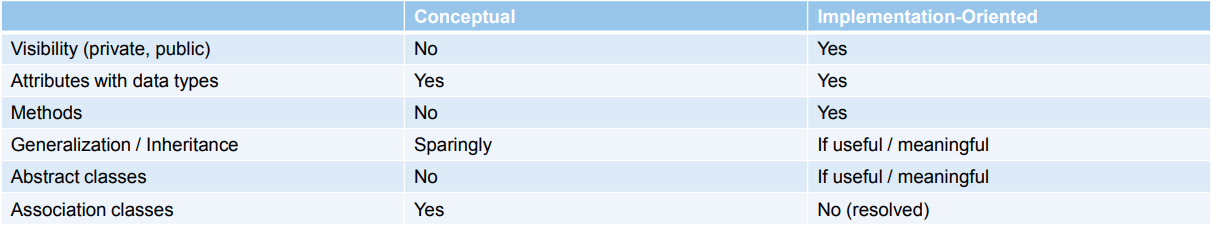
\includegraphics[width=1.0\linewidth]{umlcomparison.png}
  \label{fig:umlcomparison_png}
\end{figure}
\item \textbf{Associations between Classes:}

\pagebreak

\begin{itemize}
  \item \textbf{Multiplicity:}
	  \begin{figure}[h!]
	    \centering
	    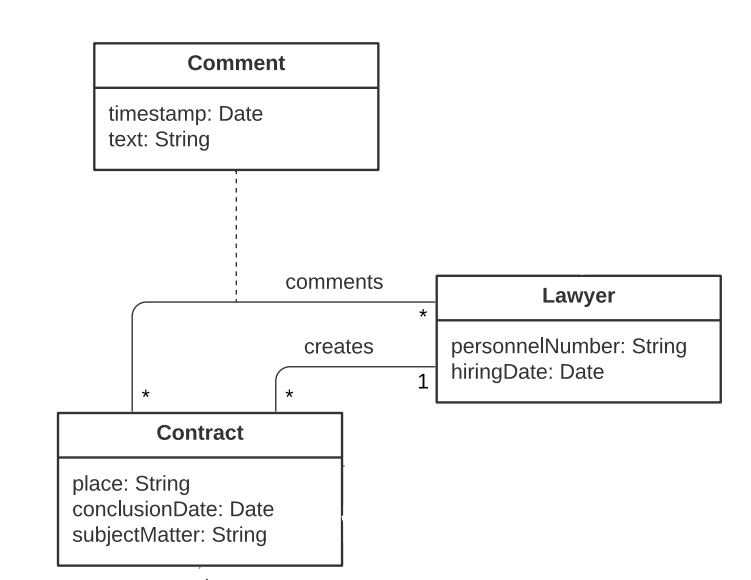
\includegraphics[width=0.5\linewidth]{umlmultiplicity.png}
	    \label{fig:umlmultiplicity_png}
	  \end{figure}
	  \\
	  \end{itemize}
	  \textit{
A Lawyer can \underline{create} \textbf{multiple} Contracts, whereas every Contract has a \textbf{single} Lawyer.
} -> \underline{creates} (action) on the side of Lawyer (actor)

\item \textbf{Aggregation:} implies a relationship where the child can exist independently of the parent (part of the parent)
\item \textbf{Composition:} implies a relationship where the child \underline{cannot exist} independent of the parent

\item  \textit{\underline{Example:}}
	\begin{figure}[h!]
	  \centering
	  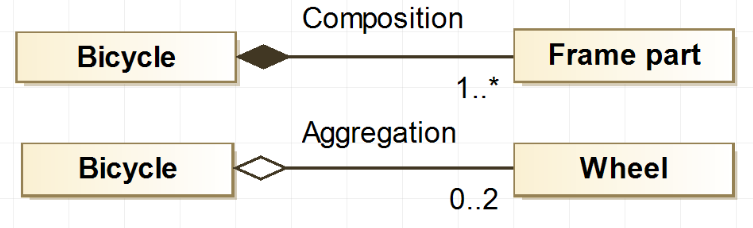
\includegraphics[width=0.4\linewidth]{compagg.png}
	  \label{fig:compagg_png}
	\end{figure}

\end{itemize}


\section{Software Estimation} % (fold)
\label{sec:software_estimation}

\subsection{Fundamentals of Estimation Methods} % (fold)
\label{sub:fundamentals_of_estimation_methods}
\begin{itemize}
  \item \textbf{Software Estimation:}
\begin{itemize}
  \item In principle, software estimation relies on \textbf{forecasting effort}, from which cost and duration are derived.
\item Regardless of the project and software methodology applied, every initiative requires the definition of a \textbf{budget} and a specific \textbf{time frame} necessary to deliver a final outcome.

\item These two are obtained during the \textbf{early stages} of the project lifecycle through the process of estimation.
\item \textbf{Estimation} aims to provide an \textbf{approximation} of the amount of recources required to complete project activities and produce a product or service in accordance to specified \textbf{functional} and \textbf{non-functional characteristics}.

\item \textbf{Software estimation conducted in early phases of the project lifecycle:}
	\begin{itemize}
	  \item necessary for contract negotiations
	\item predict expected efforts (and derived costs) for a software project before implementation
         \item best possible estimation given the available info
	\end{itemize}

\item \textbf{Agile estimation:}
	\begin{itemize}
	  \item estimation of individual requirements during project
	\item incremental allocation of developers in the most efficient manner
	\item cost estimates are made several times during development project with varying degrees of detail
	\end{itemize}
\end{itemize}
\item \textbf{Software Estimation: Cone of Uncertainty}
	\begin{itemize}
	  \item At the beginning of the project, not much is known about the product/project -> estimates underly high uncertainty
		  \item As the project progresses, more information is available -> decrease in uncertainty
	\end{itemize}
\item \textbf{Software Estimation: Costs}
	\begin{itemize}
	  \item \textbf{Cost categories:}
		  \begin{itemize}
		    \item \textbf{Development costs:} costs to produce a software product
			\item \textbf{Personnel costs:} major share of development costs for personnel
				\begin{itemize}
				  \item usually low costs for office materials etc.\ in relation to the personnel costs
				  \item proportionate allocation of CASE\footnote{Computer power-assisted software package Engineering} environment costs (including hardware and software) for product development
				\end{itemize}
		  \end{itemize}
	\end{itemize}
\end{itemize}

\subsection{Traditional Software Estimation} % (fold)
\label{sub:traditional_software_estimation}

\begin{itemize}
  \item \textbf{Sneed's Devil's Square:}
	  \begin{itemize}
	    \item Quantity
	\item Quality 
	\item Development duration
	\item Cost		
	  \end{itemize}
are mutually dependent.

\item \textbf{Quantity:}
	\begin{itemize}
		\item size of program code (example basis of assesment: LOC\footnote{Lines of Code})
		  \item functional and data scope
			  \item possible additional weighting with complexity
	\end{itemize}

\item \textbf{Quality:}
	\begin{itemize}
	  \item higher quality requirements => greater effort
	\item no \textbf{THE quality}, but different quality characteristics
	\end{itemize}

\item \textbf{Productivity:}
	\begin{itemize}
	  \item influenced by many different factors
	\item number of communication links grows \textbf{quadratically} with the team size
	\end{itemize}

\item \textbf{Development time:}
	\begin{itemize}
	  \item need more members to shorten development time
	\item more members => more communication effort
	\item higher communication => decrease in productivity
	\end{itemize}

\item \textbf{Methods for Effort Estimation:}
\begin{itemize}
  \item \textbf{Estimation Strategies:}
	  \begin{itemize}
	    \item \textbf{Top-Down:} estimation of the total project effort using mathematical algorithms based on the functional requirements
	\item \textbf{Bottom-Up:} expenses for each expense item are calculated separately and added to calculate the total project effort
	  \end{itemize}

\item \textbf{Comparison methods:}
	\begin{itemize}
	  \item estimation based on effort analysis of already accomplished similar developments
	\end{itemize}


\item \textbf{Algorithmic methods:}
	\begin{itemize}
	  \item effort calculated with algorithmic methods
	  \item based on statistical models or actual expenditure of already completed projects
	\end{itemize}

\item \textbf{Key figure methods:}
	\begin{itemize}
	  \item total cost of the software product determined by estimating the cost of individual units or project phases
	\end{itemize}

\item None of the listed basic methods alone is sufficient.
\item Depending on the point in time and knowledge of effort-relative data, one or the other method should be used.
\end{itemize}

\item \textbf{Concrete Procedures for Effort Estimation:}
	\begin{itemize}
	  \item \textbf{Goal:} Combine advantages of several effort estimation methods to deliver accurate results. (\textit{example: Function Point Method})
	\end{itemize}

\item \textbf{Function Point Method:} It is a combined relation and weighting method.
	\begin{enumerate}
	  \item \textbf{Categorization} of each product requirement (input, query, output, database, reference data)i
		  \begin{itemize}
		    \item \textbf{Input:} by the user
		\item \textbf{Output:} displaying query results, calculated data
		\item \textbf{Query:} performed on the \textbf{database} of the system, read and write
		\item \textbf{Reference data:} used to validate input, generate the output or construct the query (read-only)
		  \end{itemize}
\item \textbf{Classification} of each product requirement
	\begin{itemize}
	  \item \textbf{simple}
	  \item \textbf{medium} 
	  \item \textbf{complex} 
	\end{itemize}
	\item \textbf{Entry} into calculation form
	\item \textbf{Evaluation} of influencing factors
		\begin{itemize}
		  \item the \textbf{influence factors} refer to the application as a whole and not to individual functions or function points
		\end{itemize}
		\item \textbf{Calculation} of the evaluated Function Points (FP)
		\item \textbf{Determination} of the personnel expenses based on a FP-PM curve or table
			\begin{itemize}
				\item significant productivity decreases in large projects (FP-PM\footnote{\textbf{FP:} function points, \textbf{PM:} person month (= MM: man month)}: increase in FP => increase in PM) -> non-linear growth
			\end{itemize}
		\item \textbf{Update} of empirical data as an estimation basis for follow-up project
			\begin{itemize}
				\item After completion of a development estimated with the Function Point Method, the new value pair (FP, Actual PM) is used to update the existing curve. 
			\end{itemize}
	\end{enumerate}
\item \textbf{Function Point Method: Requirements:}
	\begin{itemize}
	  \item evaluation once the project requirements are known
	\item evaluation by employees with sufficient knowledge of requirements
\item product considered from the perspective of client
 \item company-specific training, guidelines are needed to minimize the effect of subjective individual estimates during the classification and evaluation of influencing factors
	 \item actual efforts must be measured for post-calculation
	\end{itemize}

\item \textbf{Function Point Method: Advantages}
	\begin{itemize}
	  \item product requirements, not LOC as starting point
	\item adaptability to different application areas (change of categories)
	\item adaptability to new techniques (change of influencing factors, influence evaluation)
		\item adaptability to company-specific environments (if, ie and class factors per class)
		\item refinement of the estimate according to the development process
		\item first estimate is possible at a very early stage (planning phase)
		\item good estimation accuracy
		\end{itemize}
\item \textbf{Function Point Method: Disadvantages}
	\begin{itemize}
	  \item only total effort can be estimated -> conversion to individual phases must be made using a percentage-based method
	\item personnel-intensive, not easy to automate
\item too strongly function-oriented
	\item influence factors do not clearly separate project and product characteristics
	\end{itemize}
\end{itemize}

\subsection{Agile Estimation Methods} % (fold)
\label{sub:agile_estimation_methods}

\begin{itemize}
  \item \textbf{Estimation in the SCRUM Framework:}
	  \begin{enumerate}
		  \item Estimation of \textbf{Story Points}\footnote{\textbf{Story points} are units of measure for expressing an estimate of the overall effort required to fully implement a product backlog item or any other piece of work.} for each item in the \textbf{Product Backlog}
		    \begin{itemize}
			    \item an \textbf{ordered list} of everything that is known to be needed in the product
			\item \textbf{Product Backlog Refinement:} act of adding detail, \textbf{estimates}, and order to items in the \textbf{Product Backlog}
			\item \textbf{User Story} is the unit with which software features are \textbf{estimated} and developed.
		    \end{itemize}
		\item \textbf{Time Estimation} (in days) for each item in the \textbf{Sprint Backlog}
	  \end{enumerate}

\item \textbf{Estimation with the help of Planning Poker:}
\begin{itemize}
  \item reason to use \textbf{planning poker} is to \textbf{avoid the influence of the other participants} (group thinking)
\item estimates are \textbf{story points} from different members (developers)
\item estimates are revealed simultaneously to assure the indepence between group members
\item estimates are used during \textbf{release} and \textbf{sprint planning} meetings to create release and sprint plans
\end{itemize}
\end{itemize}


% subsection agile_estimation_methods (end)


\section{Technical Foundation of Business Information System} % (fold)
\label{sec:technical_foundation_of_business_information_system}

\subsection{Architecture of Business Information Systems} % (fold)
\label{sub:architecture_of_business_information_systems}

\begin{itemize}
	\item \textbf{Architecture Patterns:}
		\begin{itemize}
			\item An \textbf{architecture pattern} describes a particular recurring design problem that arises in specific \textbf{design contexts} and presents a well-proven \textbf{generic scheme} for its solution.
			\item The solution scheme is specified by describing its constituent \textbf{components}, their \textbf{responsibilities} and \textbf{relationships}, and the ways in which they \textbf{collaborate}.
			\item \underline{\textit{Examples:}} Layered Architecture, Tiered Architecture
		\end{itemize}

\item \textbf{Layered Architectures:}
	\begin{itemize}
	  \item layers define a \textbf{logical partitioning} of software components to reduce overall system complexity
	\item \textbf{Two types of layered architectures:}
\begin{figure}[h!]
  \centering
  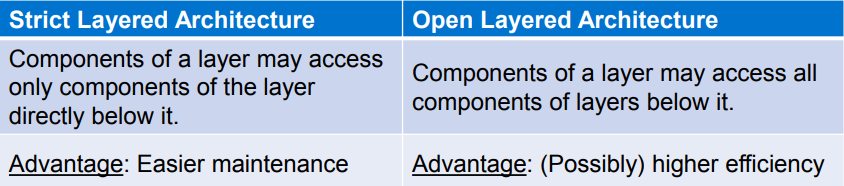
\includegraphics[width=0.6\linewidth]{layeredarchitectures.png}
  \label{fig:layeredarchitectures_png}
\end{figure}
\item a component of a layer may not access a layer above it
\item \textbf{high cohesion} between conponents within a layer, \textbf{low coupling} between different layers
\item a layer can have an explicit \textbf{interface} that distinguishes public and private components of a layer
	\end{itemize}

\item \textbf{Tiers in Architectures:}
	\begin{itemize}
	  \item Tiers define a \textbf{physical partitioning} of logical software components into different process spaces of a distributed system.

	\item a tier identifies an independent \textbf{process space} within a distributed application
	\item these process spaces can be executed on a single/different computers in a \textbf{network}
	\item each tier has a particular \textbf{responsibility} in the system and addresses a coherent set of \textbf{concerns} and \textbf{requirements} that may change over time
	\item tiers are a concept relevant for structuring software components during \textbf{execution}
	\item \textbf{n-tier architecture} defines how many tiers there are within a distributed application
	\item Typical concerns and requirements in an \textbf{information system}:
		\begin{itemize}
		  \item \textbf{Presentation Tier:} how to interact with the users?
		\item \textbf{Business Logic Tier:} how to capture and structure business logic and ensure the integrity of data?
		\item \textbf{Resource Tier:} how to persistently store and efficiently manage data?
		\end{itemize}
	\end{itemize}

\item \textbf{Client-Server Architecture:}
        \begin{itemize}
          \item two components: client and server
	\item client requests service via network protocol from server, server sends response
	\item one server can serve multiple clients
	\item a server can be a client of another server
        \end{itemize}

\item \textbf{Two-Tier Architecture:}
	\begin{itemize}
	  \item client tier and server tier
	\item assignment of tasks:
	\begin{itemize}
	  \item Presentation -> Client tier
	\item Business logic -> Client tier or server tier, both
	\item Resource management -> Server tier
	\end{itemize}
\item Advantages:
	\begin{itemize}
	  \item easy to implement
	\item high performance
	\end{itemize}
	\end{itemize}

\item \textbf{Three-Tier Architecture:}
	\begin{itemize}
	  \item Assignment of tasks:
		  \begin{itemize}
		   \item Presentation -> Client tier
	\item Business logic -> Middle tier
	\item Resource management -> Server tier
		  \end{itemize}
	\item Standard model for simple \textbf{web applications}:
		\begin{itemize}
		  \item Client tier -> HTML/CSS/JavaScript (loaded dynamically by a \textbf{browser})
		\item Middle tier -> \textbf{web application server}
		\item Server tier -> off-the-shelf \textbf{database management system}
		\end{itemize}
	\end{itemize}

\item \textbf{Four- and N-Tier Architectures:}
\begin{itemize}
  \item extension of three-tier architectures: \textbf{business logic} is distributed to several layers
\item Motivation:
	\begin{itemize}
	  \item further complexity reduction of individual tiers
	\item improved protection and isolation
	\item use of multiple and concurrent application processes
	\end{itemize}
\end{itemize}

\item \textbf{Technologies and Tiers Used in the Exercises:}
	\begin{figure}[h!]
	  \centering
	  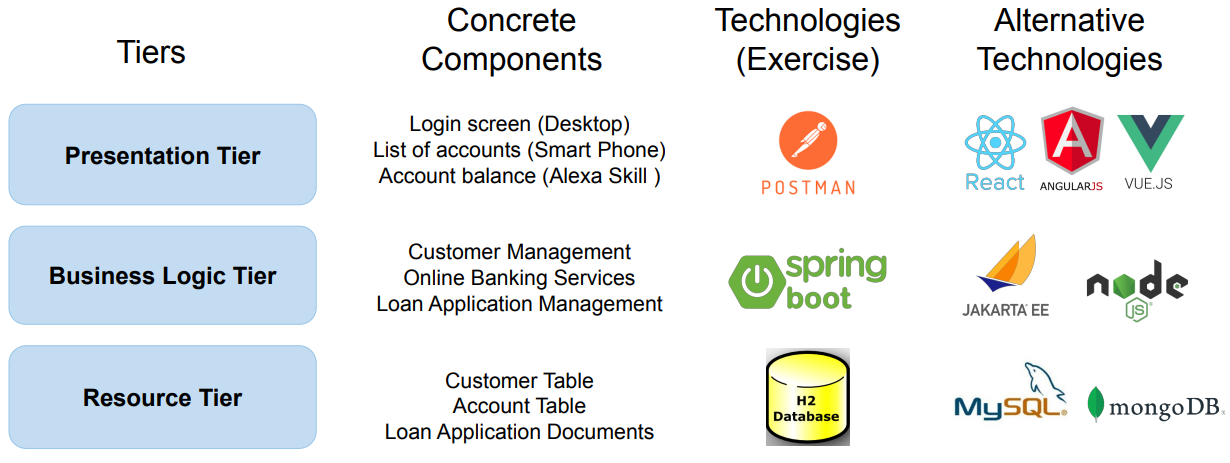
\includegraphics[width=0.7\linewidth]{techstiersex.png}
	  \label{fig:techstiersex_png}
	\end{figure}

\item \textbf{Target Architecture (SEBA Bank, SEBA Mobility Services):}
	\begin{figure}[h!]
	  \centering
	  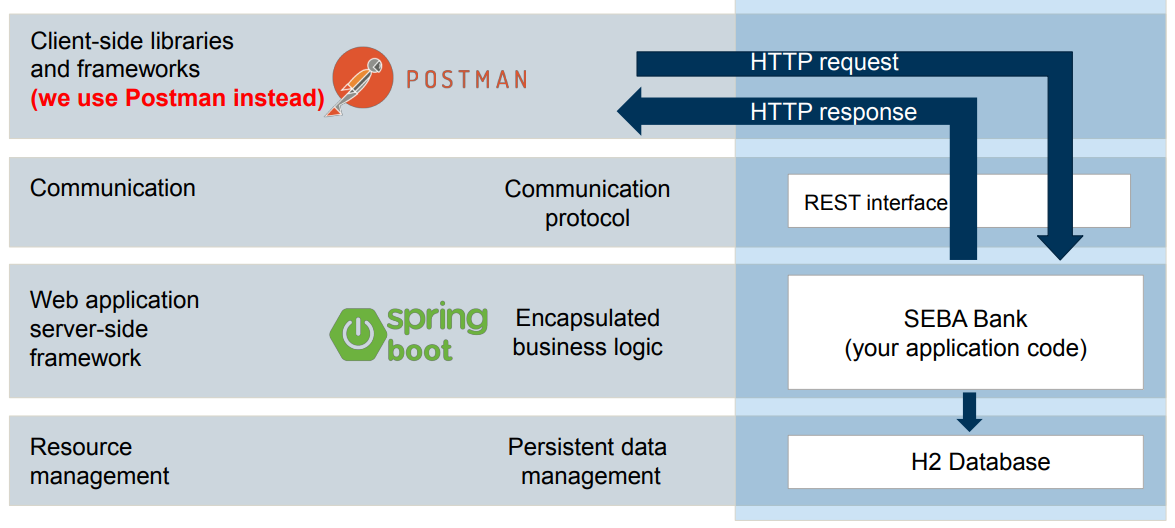
\includegraphics[width=0.8\linewidth]{targetarchitecture.png}
	  \label{fig:targetarchitecture_png}
	\end{figure}

\item \textbf{Web Server:}
	\begin{itemize}
	  \item processes incoming requests over various network protocols (HTTP)
\item provides its clients with static or dynamically generated content (HTML, CSS, files, images)
	\item \textbf{Additional tasks:}
		\begin{itemize}
		  \item resource management (sockets, static files)
		\item access control
		\item cookie\footnote{A \textbf{cookie} is a small piece of information that a website stores on your computer, and uses it at the time of your iteration on that website.} management
				\item script execution
				\item caching
		\end{itemize}
	\end{itemize}
\item \textbf{Application Server:}
\begin{itemize}
  \item web servers that execute application code to respond to HTTP requests with HTTP responses
\item enterprise software platforms offer their own application servers: Jakarta EE, SAP Web Application Server

\item \textbf{Additional tasks:}
	\begin{itemize}
	  \item authentication
		  \item authorization
			  \item session management
				  \item encapsulation of databases
					 \item transaction processing
						 \item asynchronous communication 
	\end{itemize}
\end{itemize}

\item \textbf{Database Server:}
	\begin{itemize}
	  \item \textbf{Database server (software)}
		  \begin{itemize}
		    \item software to implement data management, query optimization, concurrency control, access control
		\item can belong to different categories: Relational DB etc.
		\item provides administration tools
		  \end{itemize}

	\item \textbf{Database server (hardware)}
		\begin{itemize}
		  \item database servers usually run on a separate high-performance machines (disk IO, main memory, number of processes and threads)
		\item taking in the role of the \textbf{server}
		\end{itemize}

	\item \textbf{Used in the exercises:}
		\begin{itemize}
		  \item H2 database (relational)
		\item no separate database server / tier (embedded, in-memory)
		\item not suitable for production
		\end{itemize}
	\end{itemize}
\pagebreak
\item \textbf{Data Exchange Formats: XML and JSON:}
\begin{itemize}
  \item A \textbf{Web API} consists of a defined set of HTTP request messages.
\item for each request -> Web API specifies the structure of response messages
\item messages expressed in JSON or XML => \textbf{human-readable} data interchange
\end{itemize}
\end{itemize}


\subsection{Libraries and Frameworks} % (fold)
\label{sub:libraries_an}
\begin{itemize}
  \item \textbf{Library:} \textbf{reusable software component} that consists of several classes
	  \begin{itemize}
		  \item \textbf{functions} of the library are called by the code of the users via its \textbf{Application Programming Interface (API)}
		\item \textbf{API:} the order in which the provided functions are called is determined by the user
		\item \textit{\underline{Examples:}} Log4J (logging), JDBC (database access), dom4j (XML parsing)
	  \end{itemize}

\item \textbf{Framework:} \textbf{partially finished software system} (completed code), which consists of a variety of coordinated software components from which an \textbf{adapted software system} can be created with relatively little effort
	\begin{itemize}
		\item \textbf{Frameworks offer}
			\begin{itemize}
			  \item a basic architecture for a software system
				  \item a high degree of reusability
					\item a given set of functions that user can / have to extend
						\item whereby the general processing logic

			\end{itemize}
\item \textbf{Frameworks are tailored for specific purposes}
	\begin{itemize}
	  \item GUIs: Java Swing
	\item Web development: Spring Web
	\item Unit testing: JUnit
	\end{itemize}

\item \textit{\underline{Framework Examples:}} JUnit, Spring, Jakarta EE 
	\end{itemize}

\item \textbf{Inversion of Control (IoC):} \textbf{IoC} distinguishes a \textbf{framework} from a \textbf{library}
\begin{itemize}
	\item Since \textbf{developer} is in charge of application flow, he decides when to call the \textbf{library}. 
\item  However, when developer uses a framework, \textbf{framework} decides when to call the \textbf{library}.
\item This \underline{shift in control of calling the library} from the \textbf{application code} to the \textbf{framework} is an inversion of control.

\end{itemize}

\pagebreak

\item \textbf{Advantages and Disadvantages of Frameworks:}
	\begin{figure}[h!]
	  \centering
	  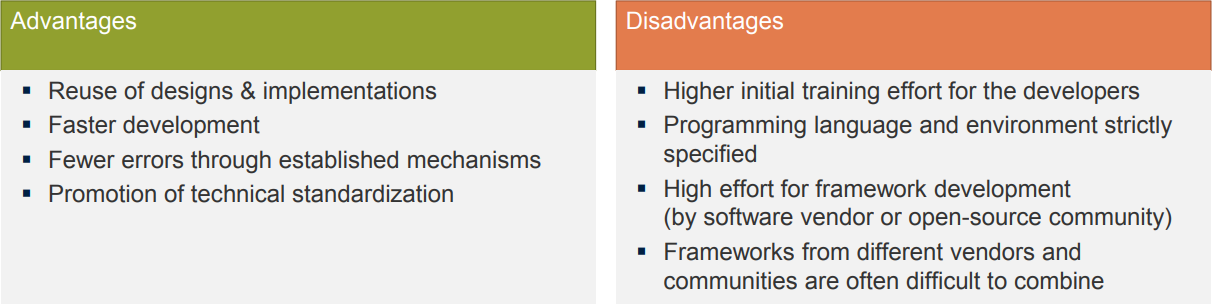
\includegraphics[width=1.0\linewidth]{addisframe.png}
	  \label{fig:addisframe_png}
	\end{figure}


\item \textbf{Jakarta EE (Framework):} a set of specifications for different purposes -> an implementation is needed to use them

\item \textbf{Spring (Framework):} a framework (configuration model) for building web applications
\begin{itemize}
  \item \textbf{Features:}
	  \begin{itemize}
	    \item IoC container with \textbf{dependency injection}
	\item data access
	\item testing
	  \end{itemize}
\end{itemize}

\item \textbf{Spring Boot:} a project within the \textbf{Spring Framework} that provides a simplified way to configure \textbf{based on conventions} and run Spring applications
	\begin{itemize}
	  \item \textbf{Motivation:} minimize amount of manual configuration (convention over configuration)

	\item \textbf{Features:}
		\begin{itemize}
		  \item creation of stand-alone Spring apps
		\item embedded web servers
		\item use of annotations
		\end{itemize}
	\end{itemize}
\end{itemize}

\subsection{Java Annotations} % (fold)
\label{sub:java_annotations}

\begin{itemize}
  \item \textbf{Motivation: Aspects and Cross-Cutting Concerns:}
	  \begin{itemize}
	    \item Software components, libraries and frameworks define \textbf{reusable code}
\item functionality separated from user code through API calls
\item user programs remain \textbf{unchanged}
\item desirable to extract \textbf{repetitive code elements} that address a certain \textbf{aspect} of overall system functionality from user programs
\item \textbf{Examples} of such aspects which address \textbf{cross-cutting concerns}\footnote{\textbf{Cross-cutting concern} relies on or affects many other aspects within that program.} of whole app:
	\begin{itemize}
	  \item component configuration and binding
	\item monitoring and logging
		\item access control
			\item data conversion for data exchange
			\item exception and transaction management
	\end{itemize}

\item \textbf{combining these aspects freely} which makes it impossible to isolate them from the user code
	  \end{itemize}

  \item \textbf{Annotation:} a tag that represents \textbf{metadata} i.e.\@  attached with class, interface, methods or fields to indicate some additional information which can be used by java compiler and JVM.

\item \textbf{Dependency Injection (DI):} a design pattern in which an object (client) receives other objects (services or dependencies) that it depends on. 
	\begin{itemize} 
	\item code that passes the service to the client is called \textbf{injector} -> injector tells client what service to use (rather than allowing client to choose)

	\item intent behind DI is to achieve \textbf{separation} of concerns of \textbf{construction} and \textbf{use} of objects
	\end{itemize}
\item \textbf{Dependency Injection in Spring (Boot):} The \textbf{injector code} is part of the framework and triggered by \textbf{annotations}.
\begin{figure}[h!]
  \centering
  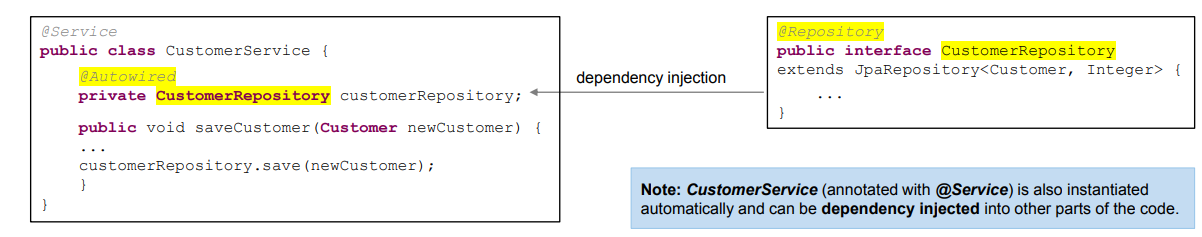
\includegraphics[width=1.0\linewidth]{dicustomer.png}
  \label{fig:dicustomer_png}
\end{figure}

\textit{\textbf{CustomerService} is the \textbf{client}, whereas \textbf{CustomerRepository} is the \textbf{service}. \textbf{@Autowired} is the \textbf{injector}.}

\item \textbf{Use of Annotations in Jakarta EE:}
\begin{itemize}
  \item Application servers or persistence frameworks like \textbf{Hibernate} provide aspects that implement the specified functionality.
\item \textit{\underline{Examples:}} \textbf{\textit{@Entity}} => for classes to be persisted into database
\end{itemize}
\item \textbf{Use of Annotations in Spring (Boot):}
	\begin{itemize}
	  \item \textbf{\textit{@Component}}: generic stereotype for any Spring-managed components\\ \\
		  \underline{Special cases of \textbf{\textit{@Component}}:}
	\item \textbf{\textit{@Controller}}: for classes at presentation layer
	\item \textbf{\textit{@Service}}: for classes at service layer
\item \textbf{\textit{@Repository}}: for classes at persistence layer\\ \\
	\underline{Other Annotations:}

\item \textbf{\textit{@SpringBootApplication}}: for Spring Boot apps
\item \textbf{\textit{@Bean}}: for objects which are created by Spring framework when the app starts (DI)
\item \textbf{\textit{@Autowired}}: for DI (automatic instantiation of specific classes (beans)) 


\end{itemize}

\item \textbf{Reflection:} process in which a program accesses info that belongs to the structure of the program itself
\begin{itemize}
  \item allows programs to examine, introspect and modify their own structure and behaviour at \textbf{compile-time} or \textbf{run-time}

\item \underline{\textit{Example:}} calling a method of an object by its name
	\begin{figure}[h!]
	  \centering
	  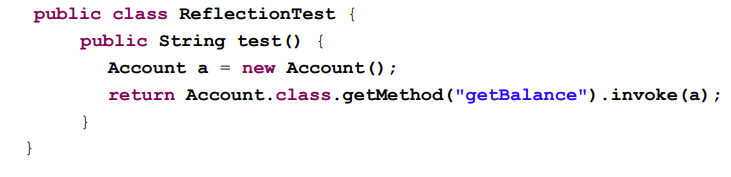
\includegraphics[width=0.7\linewidth]{reflection.png}
	  \label{fig:reflection_png}
	\end{figure}
\end{itemize}

\item \textbf{Request/Response Cycle:} \textit{Representation of a Software Application => From \textbf{Persistence Layer} (Buttom) to \textbf{Presentation Layer} (Top)}
	\begin{figure}[h!]
	  \centering
	  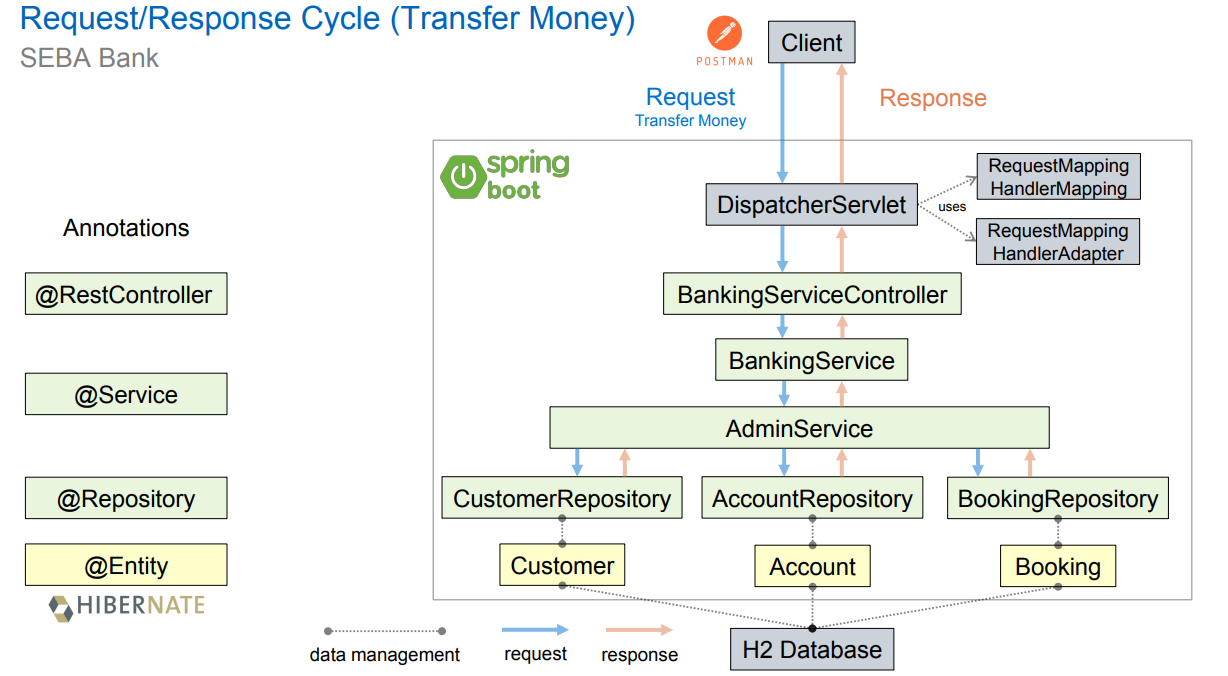
\includegraphics[width=0.7\linewidth]{reqrepcycle.png}
	  \label{fig:reqrepcycle_png}
	\end{figure}
\end{itemize}

\pagebreak
\section{Persistent Data Management} % (fold)
\label{sec:persistent_data_management}
 
\subsection{Motivation} % (fold)
\label{sub:motivation}



% subsection motivation (end)
\begin{itemize}
\item \textbf{Management of Persistent Data in Business Applications:}
		  
	  \begin{itemize}
	    \item \textbf{Persistent Data:} data that is infrequently accessed, not likely to be modified and stored beyond the lifetime of the user session (non-volatile) (e.g.\ master data, transactional data, historical data)
	  \end{itemize}

  \item \textbf{Impedance Mismatch:} a set of conceptual and technical difficulties that are often encountered because objects or class definitions must be mapped to database tables defined by a relational schema -> RDBMS\footnote{relational database management system} with object-oriented programming
	\begin{enumerate}
	  \item specialized data structures for specific access patterns
	\item relational data storage for storage of bulk data
	\end{enumerate}

\item \textbf{Databse Management Systems (DBMS):} entirety of programs for accessing database, checking consistency and modifying the data is called a database management system

	\begin{itemize}
	  \item \textbf{Persistence related functionalities:}
		  \begin{itemize}
		    \item persistent data retention
		\item modification of stored data
		\item parallel data modifications
			\item handling of mass data
				\item ensuring compliance with integrity conditions
					\item recovery in case of error
		  \end{itemize}

	\item \textbf{Variants:}
		\begin{itemize}
		  \item \textbf{Relational Database}
		\item \textbf{NoSQL Database}
		\end{itemize}
	\end{itemize}

\item \textbf{Transactions (ACID)}:
	\begin{itemize}
	  \item a \textbf{transaction} is a single unit of work, often made up of multiple operations
	\item transactions adhere to the \textbf{ACID} paradigm
	\item \textbf{ACID:}
		\begin{itemize}
		  \item \textbf{Atomicity:} entire transaction takes place at once or does not happen at all
		\item \textbf{Consistency:} database must be consistent before and after the transaction

		\item \textbf{Isolation:} multiple transactions occur independently without interference
		\item \textbf{Durability:} changes of a successful transaction occurs even if the system fails
		\end{itemize}
	\end{itemize}
\end{itemize}


\subsection{Programmatic Access to Relational Databases} % (fold)
\label{sub:programmatic_access_to_relational_databases}

\begin{itemize}
  \item \textbf{Basics of Relational Databases:}
	  \begin{itemize}
	    \item a \textbf{relational database} is a set of named tables
	\item number of rows -> cardinality of relation, number of columns -> arity of relation
	\item every relation has a \textbf{primary key} which can be a single attribute or can consist of several attributes
\item primary key of a table in another table -> \textbf{foreign key}
	  \end{itemize}

\item \textbf{H2 Database:} a relational database written in Java
	\begin{itemize}
	  \item \textbf{Main Features:}
		  \begin{itemize}
			  \item very fast, open-source, JDBC\footnote{java database connectivity} API
		\item embedded mode and server mode
			\item in-memory database -> volatile, wiped out after the execution of app
		\item browser-based console app (supports SQL)
		  \end{itemize}
	\end{itemize}
\item \textbf{Access to Persistent Relational Databases:}
	\begin{itemize}
	  \item \textbf{Goal:} business logic source code accesses persistently stored data
	\item \textbf{Common Scenario:}
		\begin{itemize}
		  \item business logic developed in object-oriented programming language
		\item relational database is used as persistent data storage

		\end{itemize}
		\item \textbf{Requirements:}
			\begin{itemize}
			  \item ACID for transactions
			\item business logic independent of data access
			\end{itemize}

		\item \textbf{Different Implementation Strategies:}
			\begin{itemize}
			  \item \textbf{Direct SQL calls:} using an applicable technology from the programming language
			\item \textbf{Software for Object-Relational Mapping:} automates aspects of access to the persistent data store
			\end{itemize}
	\end{itemize}

	\pagebreak
\item \textbf{Java Database Connectivity (JDBC): Overview}
	\begin{figure}[h!]
	  \centering
	  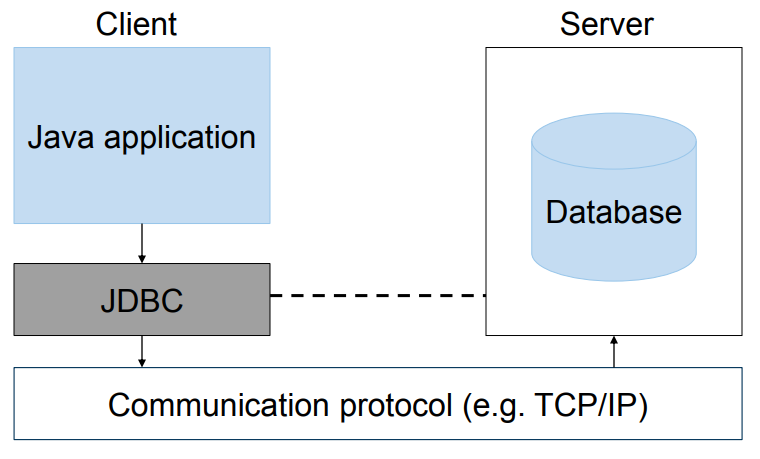
\includegraphics[width=0.4\linewidth]{jdbcoverview.png}
	  \label{fig:jdbcoverview_png}
	\end{figure}

\item \textbf{Advantages and Disadvantages of JDBC:} 
				\begin{itemize}
				  \item \textbf{Advantages:} direct use of JDBC in applications is appropriate, if
					  \begin{itemize}
					    \item stored procedures should be called
						    \item special queries have to be executed
							   \item proprietary database functionality is to be accessed
					  \end{itemize}

			\item \textbf{Disadvantages:}
				\begin{itemize}
				  \item during development often error-prune, handling is too complex for developers
				\item requires commitment to a certain persistence strategy
				\end{itemize}

			\item \textbf{JDBC calls should never be integrated directly into business logic code!}
				\end{itemize}


\item \textbf{Jakarta Persistence API (JPA):} Jakarta Persistence defines a standard API for persistent management of relational data in Java environments.
	\begin{itemize}
	  \item \textbf{Main Features:}
		  \begin{itemize}
		    \item Object-Relational Mapping (ORM)
		\item management of database access
	\item JPA itself is only a specification -> part of Jakarta EE
		  \end{itemize}
	\end{itemize}

\item \textbf{Hibernate (Framework):}
	\begin{itemize}
	  \item \textbf{Main Features:}
		  \begin{itemize}
		    \item \textbf{Object-Relational Mapping framework} for Java and RDBMS
		\item open-source
		\item full support for JPA
		\item provides an SQL-like query language: \textbf{Hibernate Query Language}
		\item serves as \textbf{abstraction above JDBC}
		\item \textbf{easy to integrate} into projects
		  \end{itemize}
	\end{itemize}
\pagebreak
\item \textbf{Object-Relational Mapping (ORM):} maps the state of objects to data in relational database to provide transparent persistent data storage and access
	\begin{figure}[h!]
	  \centering
	  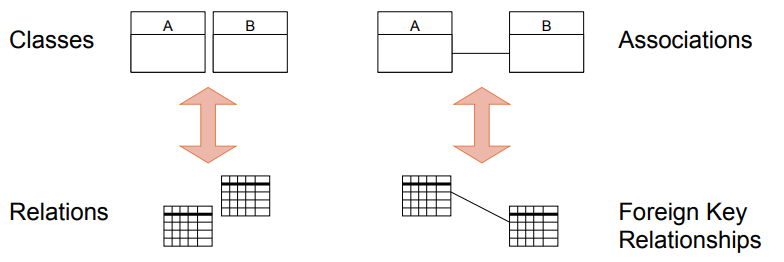
\includegraphics[width=0.5\linewidth]{orm.png}
	  \label{fig:orm_png}
	\end{figure}

\item \textbf{Software for Object-Relational Mapping:}
	\begin{itemize}
\item more complex structured transparently decomposed into flat structures of the RDBMS
\item developer sees only structures of object-oriented programming language -> transparent conversion from object-oriented operations to relational operations
	\item features already provided by RDBMS do not need to be realized by the object-oriented application again -> ensuring data integrity
	\end{itemize}

\item \textbf{Object Serialization and Deserialization:}
	\begin{itemize}
	  \item \textbf{Serialization} describes process of converting an object and all its iteratively reachable objects into a \textbf{byte or character stream} such that the object can be reconstructed through \textbf{deseerialization}.
	\item stream contains representations of attribute values, types, associations (links) between objects
	  \item can be used to store or send complex data structures
	\item not all data types can be serialized (e.g.\ threads, files) -> exception thrown
\item in Java through the interface \textit{\textbf{Serializable}}
	
	\end{itemize}
\end{itemize}

\subsection{Persistent Entities} % (fold)
\label{sub:persistent_entities}
\begin{itemize}
  \item \textbf{Basics of Persistent Entities:}
	  \begin{itemize}
	    \item Persistent Entities provide object-oriented access to the persistent info in the database (e.g.\ customer class/table).
    \item An \textbf{entity} is a persistent domain object annotated with \textit{\textbf{@Entity}}:
	    \begin{itemize}
	      \item Entity classes are mapped to tables in relational database.
		  \item Each row represents an instance of that class.
	    \end{itemize}

    \item multiple clients can use entity instances that represent the same data
	 \item each entity instance has a \textbf{unique primary key}
	\item entities exit as long as database exists (secure against server failures) or until they are deleted
	  \end{itemize}

\item \textbf{Specification/Development of an Entity:}
	\begin{itemize}
	  \item Entities obey JPA Specification:
		  \begin{itemize}
		    \item class must be annotated with \textbf{\textit{@Entity}}
		\item class must have a \textbf{default constructor} without arguments
	\item state of an entity available to clients through \textbf{entity's methods}, getters/setters
	\item class and methods must \textbf{not be final}
		  \end{itemize}

	\item Entities are annotated for ORM:
		\begin{itemize}
		  \item for entity: \textit{\textbf{@Entity}}
		\item for primary key: \textit{\textbf{@Id}}
			\item for generation of primary keys: \textit{\textbf{@GenerateValue(strategy = GenerationType.IDENTITY)}}
				\item for (re)naming a column (attribute) of table: \textit{\textbf{@Column(name = "name")}}
				\item for (re)naming a table: \textit{\textbf{@Table(name = "name")}}
				\item for enums: \textit{\textbf{@Enumerated(EnumType.STRING)}}
				\item for handling circular references: \textit{\textbf{@JsonIdentityInfo(generator = ObjectIdGenerators.PropertyGenerator.class, property = "id")}}
		\end{itemize}
	\end{itemize}


\item \textbf{Developer View of a Persistent Entity:} developer requires methods of two different types:
	\begin{enumerate}
	  \item methods to \textbf{create}, \textbf{read}, \textbf{update} and \textbf{delete} (CRUD) \underline{instances of} \underline{entities}:
		  \begin{itemize}
		    \item \textbf{EntityManager} in Jakarta
		\item \textbf{Hibernate} provides its own EntityManager called Session
		  \end{itemize}

\item methods to \textbf{read} and \textbf{update} \underline{attribute values} of an entity instance
	\end{enumerate}

\item \textbf{EntityManager:}
	\begin{itemize}
	  \item allows access to the data store by implementing programming interfaces and lifecycle rules defined by JPA
	\item associated with a persistence context, within which entity instances and their lifecycles are managed
	\end{itemize}

\item \textbf{Spring Data:} Since managing \textbf{EntityManager} manually is cumbersome, error-prone and leads to boilerplate code, Spring provides \textbf{Spring Data}

\pagebreak

\item \textbf{Spring Data and Spring Data JPA:}
	\begin{itemize}
	  \item \textbf{Spring Data:}
		  \begin{itemize}
		    \item focuses on repository abstraction
			    \item provides a familiar and consistent Spring-based programming model for data access
			\item reduces the amount of boilerplate code required to implement data access layers
\item supports Criteria API
		  \end{itemize}
	\item \textbf{Spring Data Jpa:}
		\begin{itemize}
		  \item part of larger Spring Data family, makes it easy to implement JPA-based repos
		\item not a JPA implementation but an abstraction layer to use
		\end{itemize}
	\end{itemize}
\item \textbf{Spring Data Repositories:}
	\begin{itemize}
	  \item \textbf{Annotation:} \textit{\textbf{@Repository}}
	\item Spring will detect the annotation during component scanning and \textbf{provide an instance} at runtime 
	\item \textbf{CrudRepository:} provides CRUD functions for a given entity class
	\item \textbf{PagingAndSortingRepository:} extends CrudRepository, pagination, sorting records
	\item \textbf{JpaRepository:} extends PagingAndSortingRepository, flushing/batch deleting records
	\end{itemize}

\item \textbf{Crud Repository:}
\begin{itemize}
  \item a repository must extend \textit{\textbf{JpaRepository<EntityClass, TypeOfId>}}
\item \textbf{CrudRepository} provides the methods:
	\begin{itemize}
	  \item \textbf{\textit{save()}}, \textbf{\textit{delete()}}, \textbf{\textit{findAll()}}, \textbf{\textit{findById()}}, \textbf{\textit{count()}}...
	\item \textit{\underline{Example:}}
		\begin{figure}[h!]
		  \centering
		  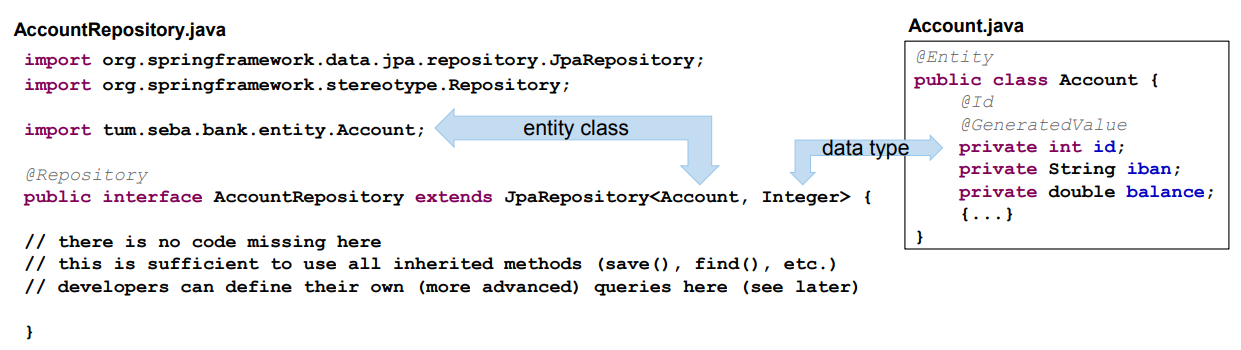
\includegraphics[width=1.0\linewidth]{repospringdata.png}
		  \label{fig:repospringdata_png}
		\end{figure}
	\end{itemize}
\end{itemize}
\pagebreak
\item \textbf{Spring Data Repositories-Advantages and Disadvantages:}
	\begin{itemize}
	  \item \textbf{Advantages:}
		  \begin{itemize}
		    \item less boilerplate code
		\item easy configuration
			\item simple queries out-of-the-box
		  \end{itemize}

		\item \textbf{Disadvantages:}
			\begin{itemize}
			  \item code is coupled to library and its specific abstractions
				  \item complete set of persistence methds are exposed -> loss of control
			\end{itemize}
	\end{itemize}

\item \textbf{Relational Mapping of Inheritance Hierarchies:}

	\begin{itemize}
	  \item \textbf{Single Table Strategy:} \textbf{\textit{@Inheritance(strategy = InheritanceType.SINGLE\_TABLE)}}
		  \begin{itemize}
		    \item \underline{all classes of inheritance hierarchy} mapped to \textbf{one (same) table}
			    \item \underline{all attributes} mapped to \textbf{colums}

				 \item \textbf{Advantages:}
					 \begin{itemize}
					   \item \underline{easy} \textbf{primary key} handling
				\item \underline{good} \textbf{polymorphic query} performance
					 \end{itemize}
\item \textbf{Disadvantages:}
	\begin{itemize}
	  \item many \textbf{NULL} values
	\item \textbf{NOT NULL} constraints on subclass entity attributes are not possible

	\end{itemize}
	\begin{figure}[h!]
	  \centering
	  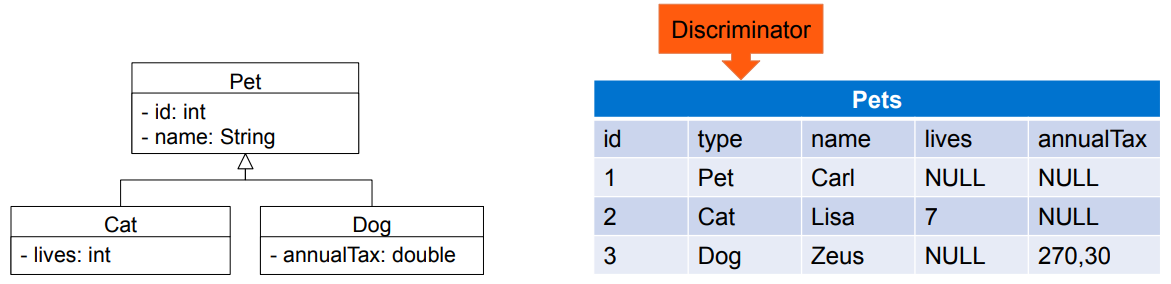
\includegraphics[width=0.7\linewidth]{singletable.png}
	  \label{fig:singletable_png}
	\end{figure}
		  \end{itemize}


\item \textbf{Joined Table Strategy:} \textit{\textbf{@Inheritance(strategy = InheritanceType.JOINED)}}
	\begin{itemize}
	  \item \underline{each class of inheritance hierarchy} mapped to \textbf{different tables}

	  \item \underline{only common attributes} in \textbf{parent's table}, \underline{subclass-specific attributes, id} in \textbf{child's table}
	\item \textbf{Advantages:}
		\begin{itemize}
		  \item \textbf{no NULL} values
		\item \underline{easy} \textbf{primary key} handling

		\end{itemize}
		\pagebreak
	\item \textbf{Disadvantages:}
		\begin{itemize}
		  \item search for instances of Pet with \textbf{JOIN}
		\end{itemize}

		\begin{figure}[h!]
		  \centering
		  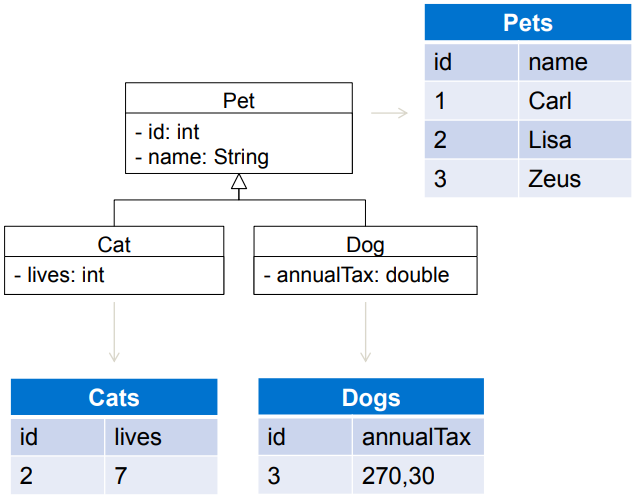
\includegraphics[width=0.4\linewidth]{joinedtable.png}
		  \label{fig:joinedtable_png}
		\end{figure}
	\end{itemize}


\item \textbf{Table per Class Strategy:} \textit{\textbf{@Inheritance(strategy = InheritanceType.TABLE\_PER\_CLASS)}}
	\begin{itemize}
	  \item \underline{each class of inheritance hierarchy} mapped to \textbf{different tables}
	  \item \underline{respective attributes} in \textbf{one table}, instances of child \textbf{not in} parent's table (nor the opposite)

	\item \textbf{Advantages:}
		\begin{itemize}
		  \item \textbf{no NULL} values
			  \item search for instances of Pet \textbf{without JOIN}
		\end{itemize}
\item \textbf{Disadvantages:}
	\begin{itemize}
	  \item \underline{complex} \textbf{primary key} handling
	\end{itemize}
	\begin{figure}[h!]
	  \centering
	  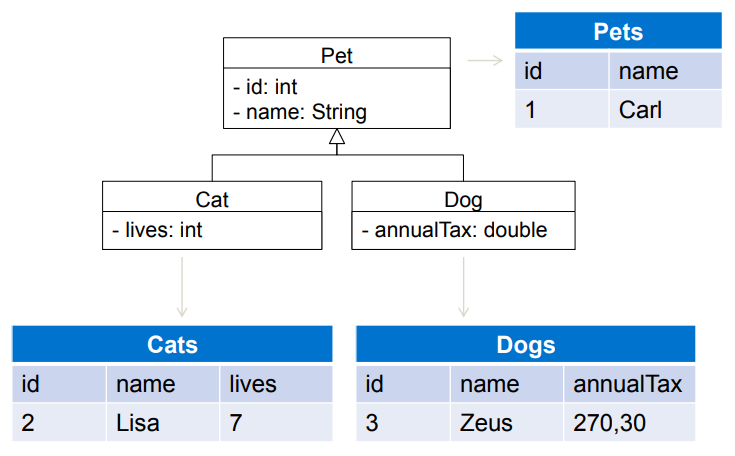
\includegraphics[width=0.4\linewidth]{tableperclass.png}
	  \label{fig:tableperclass_png}
	\end{figure}
	\end{itemize}

\item \textbf{Mapped Superclass Strategy:} \textit{\textbf{@MappedSuperclass}}
	\begin{itemize}
	  \item if parent class is \textbf{abstract}, \textbf{Mapped Suoerclass Strategy} can be used => no instances of parent
	\item \underline{each subclass} mapped to \textbf{different tables}
	\item \underline{respective attributes} in \textbf{one table}


\item \textbf{Advantages:}
	\begin{itemize}
	  \item \textbf{no NULL} values
	\item \underline{easy} \textbf{primary key} handling
\item \underline{easy way} to share \textbf{mapping info} between entities

	\end{itemize}

\item \textbf{Disadvantages:}
	\begin{itemize}
	  \item \textbf{polymorphic queries} not possible
	  \item \textbf{superclass (parent)} cannot contain associations with other entities 
	\end{itemize}
	\begin{figure}[h!]
	  \centering
	  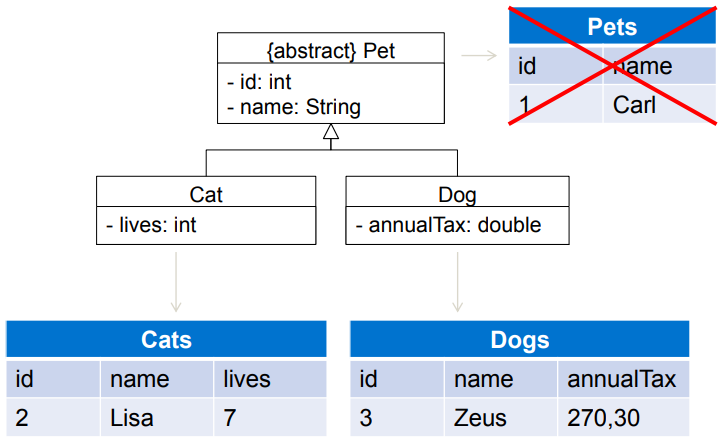
\includegraphics[width=0.4\linewidth]{mappedsuperclass.png}
	  \label{fig:mappedsuperclass_png}
	\end{figure}
	\end{itemize}
	\end{itemize}

\item \textbf{ORM for Associations Between Objects:}
	\begin{itemize}
	  \item \textbf{Associations in JPA:}
		  \begin{itemize}
		    \item \textbf{\textit{@OneToOne}}
		    \item \textbf{\textit{@OneToMany}} / \textit{\textbf{@ManyToOne}}
		\item \textbf{\textit{@ManyToMany}}
		  \end{itemize}
	\item \textbf{Parameters for update/delete propagation:} e.g.\ \textit{\textbf{@OneToOne(cascade = CascadeType.REMOVE)}}
		\item \textbf{Different loading strategies:}
			\begin{itemize}
			  \item referenced objects loaded immediately: \textit{\textbf{fetch = FetchType.EAGER}}
				  \item referenced objects loaded later on demand: \textit{\textbf{fetch = FetchType.LAZY}}
			\end{itemize}
\item \underline{\textit{Example in Java:}} \textit{\textbf{Pet} Class has the \textbf{primary key} of  \textbf{Owner} Class (mappedBy) as a \textbf{foreign key} in its table.}
	\begin{figure}[h!]
	  \centering
	  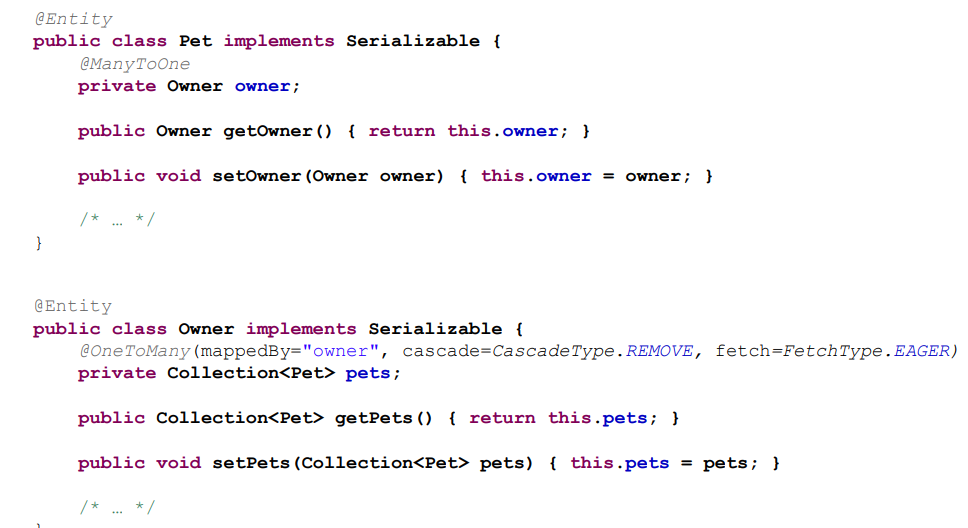
\includegraphics[width=0.7\linewidth]{onetoone.png}
	  \label{fig:onetoone_png}
	\end{figure}
	\end{itemize}

\end{itemize}

\pagebreak

\subsection{Query Languages} % (fold)
\label{sub:query_languages}
\begin{itemize}
  \item \textbf{Java Persistence Query Language (JPQL):}
	  \\ \\JPQL is not \textbf{type-safe}!
	  \begin{figure}[h!]
	    \centering
	    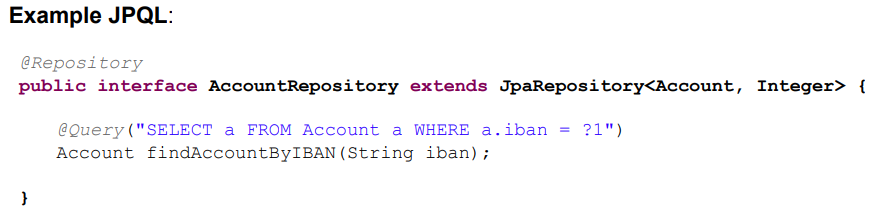
\includegraphics[width=0.7\linewidth]{examplejpql.png}
	    \label{fig:examplejpql_png}
	  \end{figure}

	  \begin{figure}[h!]
	    \centering
	    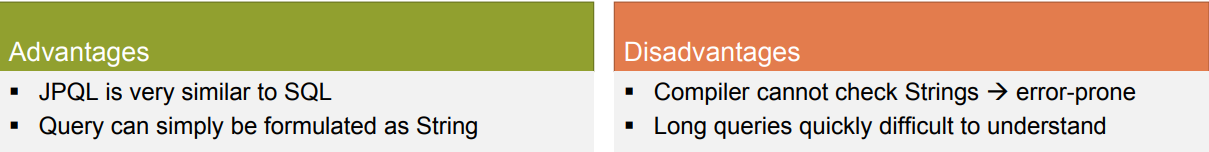
\includegraphics[width=0.7\linewidth]{addisjpql.png}
	    \label{fig:addisjpql_png}
	  \end{figure}


\item \textbf{Criteria API:}
\begin{itemize}
  \item \textbf{Motivation:}
\begin{itemize}
	  \item Neither attributes nor classes are \textbf{type-safe} in \textbf{JPQL}.
	\item Also, compiler cannot check the JPQL keywords (SELECT, FROM). 
	\end{itemize}

\item \textit{\underline{Example:}}
	\begin{figure}[h!]
	  \centering
	  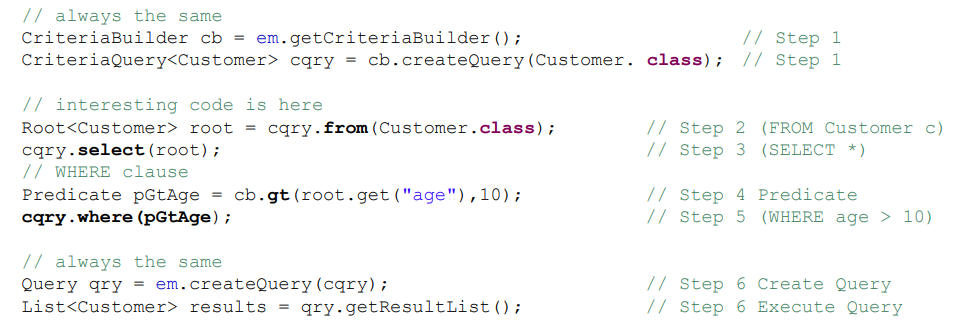
\includegraphics[width=0.7\linewidth]{examplecriteriaapi.png}
	  \label{fig:examplecriteriaapi_png}
	\end{figure}
	\begin{itemize}
	  \item \textbf{Methods for predicate definition:}
		  \begin{itemize}
		    \item \textbf{\textit{cb.gt()}}: greater than
\item \textbf{\textit{cb.equal()}}: equal
\item \textbf{\textit{cb.between()}}: between
\item \textbf{\textit{cb.and(Predicate a, Predicate b)}}: WHERE a AND b
		  \end{itemize}
	\end{itemize}
\item \textbf{Type Safety:}
	\begin{itemize}
	  \item \textbf{Type safety on attributes not yet ensured:} Reference to attribute with its name as String -> error prune
		  \begin{figure}[h!]
		    \centering
		    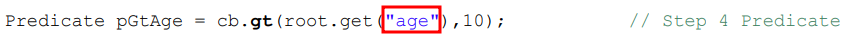
\includegraphics[width=0.7\linewidth]{criteriaapitypesafe.png}
		    \label{fig:criteriaapitypesafe_png}
		  \end{figure}
	\end{itemize}

\end{itemize}

\pagebreak
\item \textbf{Querydsl:} a framework that enables construction of statically typed SQL-like queries
	\begin{itemize}
		
	  \item \textit{\underline{Example:}}
		  \begin{figure}[h!]
		    \centering
		    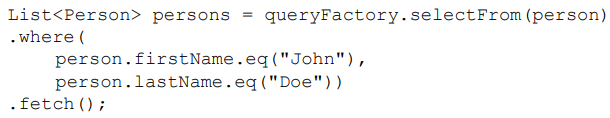
\includegraphics[width=0.7\linewidth]{examplequerydsl.png}
		    \label{fig:examplequerydsl_png}
		  \end{figure}

	\item \textbf{Advantages:}
		\begin{itemize}
		  \item more human-readable than Criteria API
		\item open-source
			\item statically typed = type-safe queries
		\end{itemize}
	\end{itemize}


\end{itemize}


\subsection{Alternatives for Persistent and Bulk Data Management} % (fold)
\label{sub:alternatives_for_persistent_and_bulk_data_management}

\begin{itemize}
  \item \textbf{NoSQL Databases:} a new generation of database systems which considers following points:
	  \begin{itemize}
	    \item associated data model \textbf{not relational}
	\item systems designed for \textbf{distributed and horizontal scalability}
	\item \textbf{schemaless} or weaker schema restrictions 
	\item due to distributed architecture, \textbf{easy data replication}
	\item \textbf{simple API}
	\item \textbf{eventually consistent}, but \textbf{not ACID}
	  \end{itemize}

\item \textbf{When to use NoSQL instead of Relational Databases:}
	\begin{itemize}
	  \item performance problems in relational databases:
		  \begin{itemize}
		    \item indexing of large amount of documents
		  \end{itemize}

	\item Relational databases are efficient if they are \textbf{optimized for frequent but small transactions} or for \textbf{large batch transactions with rare write accesses}.
	\item Relational databases are unable to handle \textbf{high data requirements} and \textbf{frequent data changes} at the same time.

	\item NoSQL databases can handle many \textbf{write} and \textbf{read} requests (e.g.\ Facebook, Amazon).
	\end{itemize}
\end{itemize}


\pagebreak
\section{Architecture of Distributed Information Systems} % (fold)
\label{sec:architecture_of_distributed_information_systems}

\subsection{Characteristics of Distributed Systems} % (fold)
\label{sub:characteristics_of_distributed_systems}

\begin{itemize}
  \item \textbf{Foundations:}
	  \begin{itemize}

	\item \textbf{Distributed system:} a system that is comprised of several physically disjoint compute resources interconnected by a network
	    \item \textbf{Distributed Application:} an application consisting of severeal processes that run distributed in several process spaces
\item \textbf{Characteristics of a distributed system:}
	\begin{itemize}
	  \item resource sharing
	\item openness (communication protocols and interfaces)
	\item concurrency
		\item scalability
			\item failure tolerance
				\item distribution transparency
	\end{itemize}
	  \end{itemize}
\item \textbf{A Centralized Information System Architecture:}
\begin{itemize}
  \item \textit{\underline{Example:}} Central mainframe
	  \begin{itemize}
	    \item multi-user operation
	\item optimized for large amounts of data
		\item high reliability
		\item minimal logic on the terminal, only display of data
	  \end{itemize}
\end{itemize}
\item \textbf{A Local Area Network of Distributed Clients and Servers:}
	\begin{itemize}
	  \item distributed system within a company, department
		  \begin{itemize}
		    \item multi-user operation
		\item distributed services and information
		  \end{itemize}

	\item different functionalities supported by different servers
		\item automation of business processes
		\item requirement of integration effort and leads to \textbf{productivity paradox}:
			\begin{itemize}
			  \item more IT investments do not lead to higher productivity
				  \item limited realization of compound effects
			\end{itemize}
	\end{itemize}

\item \textbf{Resource Sharing:}
	\begin{itemize}
	  \item \textbf{client-server model} -> based on service-oriented achitecture for resource sharing
	\item \textbf{server} processes provide \textbf{resource managers}, they provide shared resources (e.g.\ data, code, hardware, processes)
\item \textbf{client} processes issue requests to use these remote resources
\item client initiates the communication
	\end{itemize}

\item \textbf{Opennes and Concurrency:}
	\begin{itemize}
	  \item \textbf{Openness}
		  \begin{itemize}
		    \item extensibility of the system at the
			   \begin{itemize}
			     \item \textbf{hardware level:} new peripherals, memory, etc.
			\item \textbf{software level:} new resource services, communication protocols
			   \end{itemize}
		\item specifications for \textbf{interfaces} of the system are disclosed and documented
		  \end{itemize}

\item \textbf{Concurrency:}
	\begin{itemize}
	  \item multiple users issue independent and concurrent requests via client processes
\item server processes run concurrently
	\item multiple processes may exist for each resource type to improve scalability
	\end{itemize}

	\end{itemize}
\item \textbf{Scalability and Failure Tolerance:}
	\begin{itemize}
	  \item \textbf{Scalability}
		  \begin{itemize}
		    \item adapting the system for larger data volumes, workloads, faster throughput
		\item increase in complexity
		\item ideally without changing application architecture
		\item \textbf{Goal:} constant performance with increasing load
		  \end{itemize}

\item \textbf{Failure tolerance}
	\begin{itemize}
	  \item ability of distributed system to provide functionalities even if a number of defective subsystems (servers/clients) exist
\item implementation via redundant subsystems, a certain number of which can be defective
\item guarantee of high availability
	\end{itemize}
	\end{itemize}

\item \textbf{Transparency:}
	\begin{itemize}
	  \item \textbf{distributed system apppears as a single computer system} -> structure hidden from programmer
	\item \textbf{Forms of transparency}
		\begin{itemize}
		  \item 
		\end{itemize}
	\end{itemize}
\end{itemize}

% subsection characteristics_of_distributed_systems (end)

% section architecture_of_distributed_information_systems (end)

% subsection alternatives_for_persistent_and_bulk_data_management (end)


% subsection query_languages (end)
% subsection persistent_entities (end)























% subsection programmatic_access_to_relational_databases (end)
% section persistent_data_management (end)
% subsection java_annotations (end)
% subsection libraries_an (end)
% subsection architecture_of_business_information_systems (end)

% section technical_foundation_of_business_information_system (end)





% subsection traditional_software_estimation (end)

% subsection fundamentals_of_estimation_methods (end)

% section software_estimation (end)















% section conceptual_modeling_with_uML (end)




% subsection interactive_requirements_collection (end)
% subsection traditional_requirements_engineering (end)
% section requirements_engineering (end)
% subsection characteristics_of_business_applications (end)

% subsection standard_and_custom_software ()

% subsection classification_of_business_applications (end)


% subsection business_without_iT_support (end)

% section iT_support_for_business_applications (end)



\end{document}
